\documentclass[10pt,a4paper]{article}
%\usepackage{hyperlatex}
\usepackage{graphicx}
\usepackage{listings}
\usepackage{geometry}
\usepackage{html}
\usepackage{verbatim}

\geometry{left=2.5cm, right=2.5cm, bottom=2cm, top=2cm}
%\htmltitle{KPilot Conduits programming tutorial}
%\htmladdress{\xlink{Reinhold Kainhofer}{mailto:reinhold@kainhofer.com}, 
%\htmladdnormallink{http://reinhold.kainhofer.com}{http://reinhold.kainhofer.com/} \today}
%\htmlattributes{BODY}{BGCOLOR=#ffffee text=#000000 link=#0000FF vlink=#000099 alink=#000099}


%\setcounter{htmldepth}{2}
%\setcounter{secnumdepth}{4}

\title{KPilot conduit programming tutorial}
\author{\htmladdnormallink{Reinhold Kainhofer}{mailto:reinhold@kainhofer.com}, with help of 
\htmladdnormallink{A. de Groot}{mailto:groot@kde.org} and \htmladdnormallink{Dan Pilone}{mailto:pilone@slac.com}}
\date{\today}

%\W \newcommand{\texttrademark}{}
\newcommand{\code}[1]{{\small\texttt{#1}}}
\newcommand{\file}[1]{{\small\texttt{#1}}}
\newcommand{\class}[1]{{\small\em\texttt{#1}}}

\newcommand{\codesize}[0]{\scriptsize}

\begin{document}

\maketitle


%\htmlmenu{3} 

\tableofcontents 



\section{Introduction and General}

\subsection{Introduction}
    One of the greatest assets of the handheld computers is their ability to
interconnect with other applications.  KPilot supports this capability
through conduits.  A conduit is a small separate program that talks to
KPilot during the hot sync.  The conduit translates between the Palm
Pilot and the application you're syncing with.

For KPilot to be a really usable synchronization application, it depends
on third-party developers to enlarge the conduit gallery to other applications. In particular, I want to encourage developers of Palm applications to provide not only a Windows\texttrademark conduit, but at the same time put some effort in providing also a conduit for Linux and other platforms.
This is also the reason why I'm writing this tutorial: 
To encourage third-party developers to write conduits for KPilot. 

I will show the process at several examples: \\
First, the general framework (library, factory etc.) for a conduit is presented 
in section \ref{FactorySection}, then in section \ref{SetupSection}. 
I will describe how you can write a configuration dialog for your conduit. These 
two sections will use the malconduit (AvantGo conduit) as an example. 
The synchronization part (the conduit class) will be described in the next few 
sections. Section \ref{SectionSimpleConduit} will show a very simple 
synchronization at the example of the AvantGo conduit, where we will use the 
functions of an external library which will do the synchronization for us. 
In section \ref{SectionDatabasesConduit} I will show a synchronization process 
where one file on disk corresponds to one database on the palm, and where no conflict 
resolution and no record comparison needs to be done, because we have to copy the 
whole database either from or to the handheld. The particular example there will be the docconduit which 
synchronizes text files on the harddisk with PalmDOC documents for AportisDoc, TealDoc, MobiPocket Reader, Gutenpalm etc. 
on the Palm.
Finally, I wanted to show an example of a record-based conduit, but then decided it 
would be too extensive to replicate all the complex sync and conflict resolution code.
Instead I refer to the addressbook conduit, which you should be able to understand 
quite well after studying the other conduits explained in the previous chapters of this How-To.
Using KDE's KitchenSync general synchronization framework for syncing will be the topic of section 
\ref{SectionKitchenSync}, where I give some argument why we do not yet switch to kitchensync yet.

\subsection{Further information and links}

There are loads of information about the PalmOS\texttrademark Database format 
out there:
\begin{itemize}
\item Palm's official Developer Knowledge Base document: \htmladdnormallink{http://oasis.palm.com/dev/kb/faq/FileFormat/PDB+PRCFormat.cfm}{http://oasis.palm.com/dev/kb/faq/FileFormat/PDB+PRCFormat.cfm}
\item PilotRecord Databse format: \htmladdnormallink{http://www.pda-parade.com/prog/palm/doc/pdb.html}{http://www.pda-parade.com/prog/palm/doc/pdb.html}
\item EBNF representation of the database format: \htmladdnormallink{http://obermuhlner.com/public/Projects/Palm/PDBC/Documentation/pdbc\_file.html}{http://obermuhlner.com/public/Projects/Palm/PDBC/Documentation/pdbc\_file.html}
\item A list of several Palm databse formats: \htmladdnormallink{http://myfileformats.com/search.php?name=Palm}{http://myfileformats.com/search.php?name=Palm}
\end{itemize}

\subsection{Legal}
You can skip this chapter if you are familiar with HOWTOs,
or just hate to read all this assembly-unrelated crap.

\subsubsection{Legal Blurb}

Permission is granted to copy, distribute and/or modify this document
under the terms of the GNU \htmladdnormallink{Free Documentation
License}{http://www.gnu.org/copyleft/fdl.html}  Version 1.1;
with no Invariant Sections, with no Front-Cover Texts, and no Back-Cover texts.
A copy of the license is included in the \htmladdnormallink{Free Documentation
License}{http://www.gnu.org/copyleft/fdl.html} appendix.


The most recent official version of this document is available from
\htmladdnormallink{my homepage}{http://reinhold.kainhofer.com/Linux/KPilot/ConduitTutorial}.
If you are reading a few-months-old copy,
consider checking the above URLs for a new version.



\section{The general conduit framework}\label{FactorySection}

\subsection{How conduits work in general}
    KPilot is divided into three major components: the GUI, the
syncing daemon, and the conduits.  When the GUI is started it attempts
to make a connection to the syncing daemon.  If it can't it starts the
daemon then makes the socket connection.  When the user hits the
hot-sync button on the cradle the daemon checks to see if the GUI is
connected.  If it is, the daemon notifies the GUI that a hot-sync has
started.  The daemon then steps through all activated conduits and lets them
do their sync. When the conduit is started it
makes a connection back to the daemon and asks the daemon to read and
write entries into the database.  When the conduit finishes it exits
and the daemon continues on to the next conduit.  Once all the
conduits have run the daemon alerts the GUI that it has
finished and goes back to waiting for a sync to start. Note that the backup 
of the Handheld is also done by a conduit, which is not visible to the user, though.


    The basic conduit implements three important features:
info/setup, backup, and normal hot-sync.  If the user clicks the setup 
button in KPilot's conduit menu the conduit is started and requested
to show a settings dialog.  If the conduit doesn't have any settings
to adjust then it should simply display an about dialog.  When the
dialog is closed the conduit will exit.  Next, if the user requested
KPilot back up the pilot the conduit will be given the opportunity to
grab everything off the pilot.  This is useful if this is the first
time the conduit is being used.  For example if the user had never
synced before this would be a good time to copy the data into the
calendar, money database, etc.  Lastly, the conduit is requested to
hot-sync whenever KPilot is hot-syncing with the pilot. 



\subsection{A conduit is a KDE shared library}

From your system's point of view, a conduit is a shared library which is loaded 
on demand by KPilot. This means that as long as you don't do a sync, the conduit will not 
be in memory. Once a hotsync is initiated, kpilotDaemon (the process running in 
the background that does the actual sync) loads the conduit, let's say its name 
is "malconduit" and it is installed as /opt/kde3/lib/kde3/libmalconduit.so. It 
then calls the function \code{init\_libmalconduit} (the name after init\_ is the 
filename of the library), which needs to return a pointer to an instance 
of a \class{KLibFactory} subclass. 

{\small\begin{verbatim}
extern "C" {

void *init_libmalconduit() {
    return new MALConduitFactory;
}

};
\end{verbatim}
}

Whenever the conduit needs to do some action 
(show the configure dialog or do a sync), the \code{createObject(...)} method 
of this instance is called with the appropriate values to specify the action. It either returns an instance 
of a \class{ConduitConfig} subclass to show the configuration dialog, or an 
instance of an \class{ConduitAction} subclass which will later do the actual sync 
with the handheld. Figure \ref{ConduitStructure} shows this as a diagram:

\begin{figure}
\begin{center}
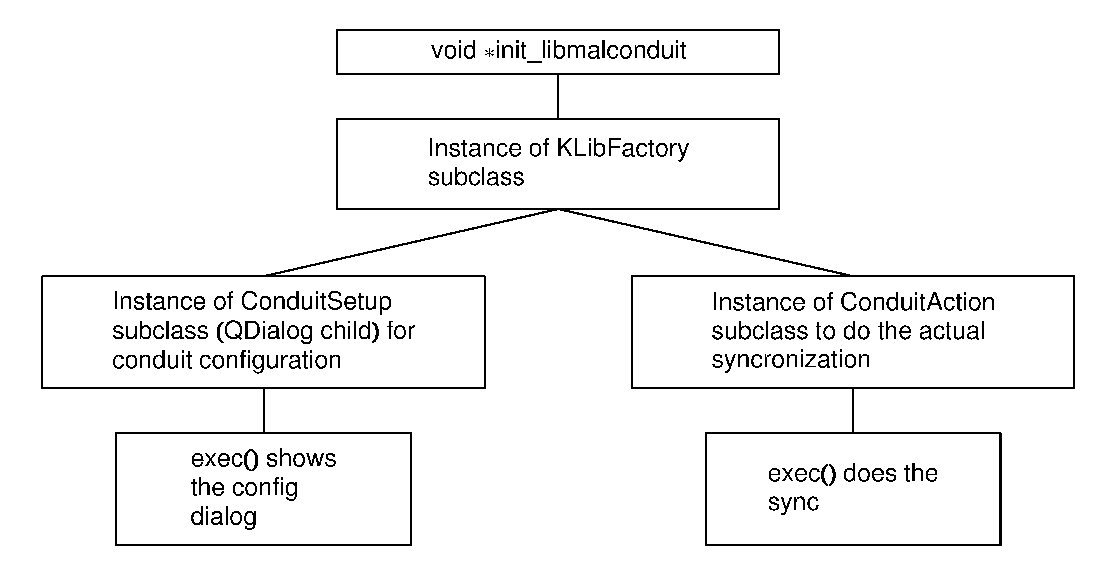
\includegraphics[width=13cm]{ConduitStructure}
\caption{The general structure of a conduit}\label{ConduitStructure}
\end{center}
\end{figure}


\subsection{Makefile.am and KDE build process}

Before we delve into programming details, let us look a bit at the compilation framework.

If you develop your conduit inside the \file{kdepim/kpilot/conduits} directory of KDE's 
CVS tree, all you need to do is to provide a Makefile.am in your conduit directory 
(e.g. \file{kdepim/kpilot/conduits/malconduit}), and add the name of your 
directory (\file{malconduit} in this example) to the variable \code{SUBDIRS} 
in \file{kdepim/kpilot/conduits/Makefile.am}:
{\small
\begin{verbatim}
SUBDIRS = knotes expense null vcalconduit \
          popmail timeconduit malconduit
\end{verbatim}
}
\vspace{1em}

The \file{Makefile.am} in your conduit's directory will look similar to the following one 
(taken from the malconduit). Since this is a tutorial on KPilot conduits, and not 
on automake/conf, make and Makefiles, I will not explain it in detail. However, 
it should be easy to adapt it to your conduit's needs:

{\footnotesize
\begin{verbatim}
### Makefile for the AvantGo conduit
###
### The mal conduit is Copyright (C) 2002 by Reinhold Kainhofer


INCLUDES= $(PISOCK_INCLUDE)  $(MAL_INCLUDE) \
  -I$(top_srcdir)/kpilot/lib $(all_includes)
METASOURCES = AUTO

servicedir = $(kde_servicesdir)
service_DATA = mal_conduit.desktop

kde_module_LTLIBRARIES = libmalconduit.la

libmalconduit_la_SOURCES = \
        mal-factory.cc \
        mal-setup.cc \
        mal-conduit.cc \
        mal-setup_dialog.ui
libmalconduit_la_LDFLAGS = $(KDE_RPATH) -L../../lib
libmalconduit_la_LIBADD = -lkpilot $(MAL_LIB)
\end{verbatim}
}

Here is a short table of the variables used in \file{Makefile.am}:

\begin{tabular}{ll}
\code{service\_DATA} & name of the desktop file of your conduit \\
        &(tells KDE which library it needs to load)\\
\code{kde\_module\_LTLIBRARIES} & tell make which libraries to compile\\
\code{libraryname\_SOURCES} & a list of all source files to be compiled into \\
        &libraryname (where a . is replaced by a \_)\\
\code{libraryname\_LDFLAGS} & linker flags when linking your conduit \\
\code{libraryname\_LIBADD} & additional libraries the conduit links to \\
        &(-lkpilot is the KPilot base library and\\
        & needs to be linked to every conduit)
\end{tabular}

\vspace{0.5em}

Both \code{MAL\_INCLUDE} and \code{MAL\_LIB} are special variables 
pointing to the headers and the library of libmal, and are set by 
\file{configure.in.in} (see below).

\vspace{1em}

If you have special library requirements (e.g. the malconduit needs libmal to work), 
you need to add special configure checks to the autoconf file \file{kdepim/kpilot/conduits/configure.in.in} (for an 
example, you should look at the checks the malconduit added to the file in CVS) 
and include the directory only if the appropriate libraries and header files are installed. 
One way to achieve this is to add the following line after your configure checks, which set 
the variable \code{HAVE\_MAL} to \code{1}. This automake command in 
\file{configure.in.in} defines "\code{include\_malconduit}" for use 
in Makefile.am, if \code{HAVE\_MAL==1}:
{\small\begin{verbatim}
AM_CONDITIONAL(include_malconduit, test "$HAVE_MAL" = "1")
\end{verbatim}
}

You can then use "\code{include\_malconduit}" in the KPilot conduit 
directory's makefile \file{kdepim/kpilot/conduits/Makefile.am}:
{\footnotesize
\begin{verbatim}
MALSUBDIR=
if include_malconduit
    MALSUBDIR = malconduit
endif

SUBDIRS = knotes expense null vcalconduit popmail timeconduit $(MALSUBDIR)
\end{verbatim}
}

\subsection{The conduit factory}

In KDE's dynamic library system, the library factory plays a crucial rule. The \code{init\_libraryname()} function 
always returns a pointer to a \class{KLibFactory} instance. Whenever a program needs a special action by 
the conduit, it calls the \code{createObject} of the \class{KLibFactory} to get an appropriate object.
Furthermore, the conduit factory initializes the about dialog of the conduit. 

The factories of all conduits are very similar, so you best just copy the .h and .cc file of an existing conduit 
for your conduit. All you need to do is to change the copyright notices for the about dialog, and 
change the class names of the \class{ConduitAction} and \class{ConduitSetup} to your own class names. Also, 
the factory is a good place to define the strings for the config settings' entries to the config file.
If you define them like:
{\footnotesize\begin{verbatim}
class MALConduitFactory : public KLibFactory
{
...
public:
    static const char *configSetting1() {return fConfigSetting1;};
private:
    static const char *fConfigSetting1;
} ;
\end{verbatim}
}
and in the .cc file
{\small\begin{verbatim}
const char*MALConduitFactory::fConfigSetting1="NameOfSetting";
\end{verbatim}
}
you can use them as \code{MALConduitFactory::configSetting1()} in 
both the configuration dialog and the sync routine without running the risk of misspelling
them.

Everything else in the factory can stay as it is.

Here is an example of the malsync's factory:
\begin{htmlonly}
  \htmladdnormallink{Source code of mal-factory.h}{mal-factory.h}
  \htmladdnormallink{Source code of mal-factory.cc}{mal-factory.cc}
\end{htmlonly}


\begin{latexonly}
\subsubsection{mal-factory.h}
{\scriptsize
 \verbatiminput{mal-factory.h}
}
\subsubsection{mal-factory.cc}
{\scriptsize
 \verbatiminput{mal-factory.cc}
}
\end{latexonly}

\subsection{Debugging conduits}

Debugging KPilot conduits is not an easy task, as one cannot use a debugger 
(because conduits are shared libraries and kpilotDaemon forks itself 
in the background when it is started).

So printing debug output is the only way to get any information about what 
the conduit is doing. If you don't configure kdepim it with \code{--no-debug}, or don't add 
\code{--NDEBUG} in Makefile.am, then you can easily print out debug messages
using the \code{DEBUGCONDUIT} stream. However, at the beginning of each 
function where you want to use it, you need to add the macro \code{FUNCTIONSETUP;}, 
which prints out a debug message with the current function name. Additionally, 
it sets several variables like \code{fname} which holds the name of the current function.

 As an example, the following code
{\footnotesize\begin{verbatim}
void YourConduit::somefunction() {
    FUNCTIONSETUP;
    int i=5;
#ifdef DEBUG
    DEBUGCONDUIT<<fname<<": Value of i="<<i<<endl;
#endif
}
\end{verbatim}
}
prints out the following debug message to stdout:
{\small\begin{verbatim}
kpilotdaemon: somefunction: Value of i=5
\end{verbatim}
}



\section{The Conduit Setup Dialog}\label{SetupSection}

In this section I will shortly describe how you can implement a configuration dialog for your conduit. 
There is nothing Palm- or KPilot-specific about this. All the configuration dialog does is to read the 
configuration settings from the config file (using the \class{KConfig} class from kdelibs), and let 
the user change them in the dialog. If the user exists the dialog by pressing OK, the new values are 
read from the dialog controls and written back to the configuration file.

To provide a consistent experience to KPilot users, there already 
exists a class \class{ConduitConfig} which is a subclass of \class{KDialog}. 
This dialog does most of the basic work for you.

\subsection{The dialog template, using QT Designer}
Of course, first we need to have a dialog template in the form of a QT 
Designer file (which has an extension .ui). Start up \file{designer} and 
create a new widget (no dialogbox, i.e. no OK or cancel buttons, these will be added automatically). The dialogbox should contain a QTabWidget, even if you only need one tab. A second tab "About" will be added more or less automatically by the conduit listing the copyright and the authors of your conduit. A typical example of the coknduit setup widget dialog is shown in the following screenshot:
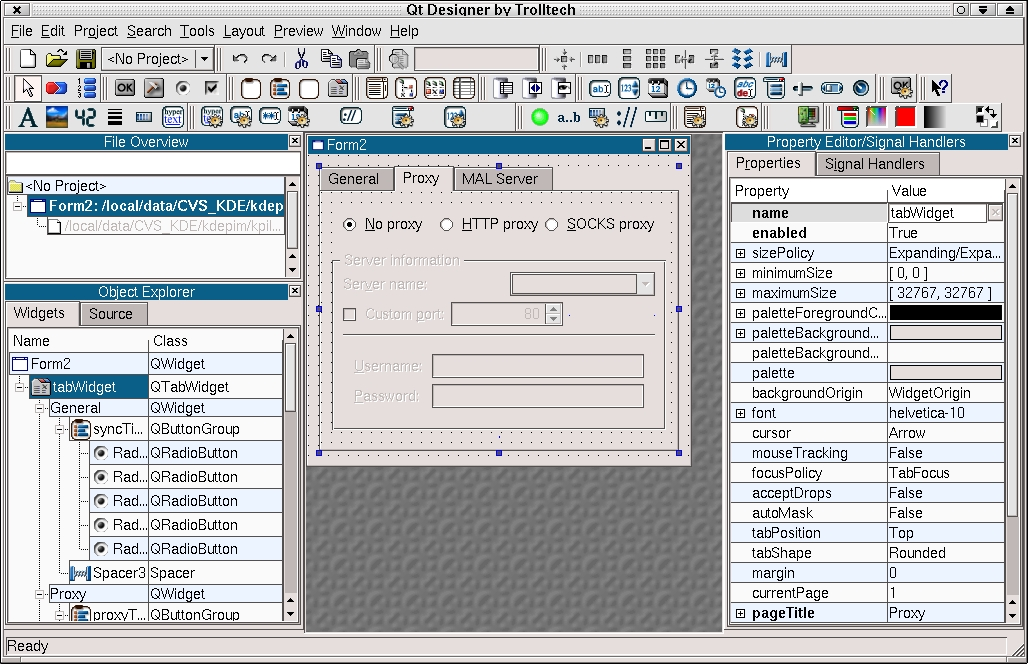
\includegraphics[width=14cm]{pictures/ProxyTab}


\subsection{Using the dialog template for your conduit}

Now that we have the dialog template, we can include it in the configuration dialog box. 
First, create a subclass of \class{ConduitConfig}, where we only have to implement the con- and 
destructor as well as the methods
\begin{itemize}
\item \code{virtual void readSettings()} 
\item \code{virtual void commitChanges()}
\end{itemize}
This class \class{ConduitConfig} will do most of the work for us, all 
that is left to us is to read the config settings from the config file 
and set the values of the controls in the dialog (in the 
\code{readSettings()} method). Also, when \code{commitChanges()} is 
called, this means that the dialog was existed with the OK button, so 
we need to read the new values from the controls and store them to the 
configuration file.

The whole class declaration is:
{\footnotesize\begin{verbatim}
class MALWidget;

class MALWidgetSetup : public ConduitConfig 
{
Q_OBJECT
public:
    MALWidgetSetup(QWidget *,const char *,const QStringList &);
    virtual ~MALWidgetSetup() {};
    virtual void readSettings();
protected:
    virtual void commitChanges();
private:
    MALWidget *fConfigWidget;
} ;
\end{verbatim}
}

This class implements the dialog box itself, and our dialog template 
will be inserted into this dialog by the constructor:
{\footnotesize\begin{verbatim}
MALWidgetSetup::MALWidgetSetup(QWidget *w, const char *n,
    const QStringList & a) :
    ConduitConfig(w,n,a)
{
    FUNCTIONSETUP;

    fConfigWidget = new MALWidget(widget());
    setTabWidget(fConfigWidget->tabWidget);
    addAboutPage(false,MALConduitFactory::about());

    fConfigWidget->tabWidget->adjustSize();
    fConfigWidget->resize(fConfigWidget->tabWidget->size());
}
\end{verbatim}
}

The first two lines create an instance of our dialog template and add it 
as the tab widget to the dialog. Since we will have to set and read the 
values of the controls in that tab widget, we need to store a pointer to 
the instance in the variable \code{fConfigWidget} which is of the same type 
(\code{MALWidget}) we assigned to our dialog template in QT Designer. The 
third line of code adds the about page (which is created by the factory, 
see last section) to the tab widget, while the last two line just adjust 
the size of the dialog box and are not always needed.

As mentioned above, we only need to implement \code{MALWidgetSetup::readSettings()} 
and \code{MALWidgetSetup::commitChanges()}. The \class{ConduitConfig} class 
already stores an instance named fConfig to KPilot's configuration facility. 
We only have to set the correct configuration group name (I suggest, you 
store the name of the configuration group for you conduit in a \code{static 
char*} variable of the conduit factory class), and then we can use the methods
\begin{itemize}
\item \code{fConfig->readEntry("entryname", \em{defaultNumericValue})}
\item \code{fConfig->readEntry("entryname", \em{defaultstring})}
\item \code{fConfig->readBoolEntry("entryname", \em{defaultBoolValue})}
\end{itemize}
to retrieve the settings from the configuration file. We then use the methods of the QT and KDE widgets to assign the text or value to the controls:

{\footnotesize\begin{verbatim}
/* virtual */ void MALWidgetSetup::readSettings()
{
    FUNCTIONSETUP;

    if (!fConfig) return;
    KConfigGroupSaver s(fConfig,MALConduitFactory::group());
    
    fConfigWidget->syncTime->setButton(fConfig->readEntry(MALConduitFactory::syncTime(), 0));
    
    // Proxy settings
    fConfigWidget->proxyType->setButton(
        fConfig->readEntry(MALConduitFactory::proxyType(), 0));
    fConfigWidget->proxyServerName->setEditText(
        fConfig->readEntry(MALConduitFactory::proxyServer(), ""));
    int proxyPortNr=fConfig->readEntry(MALConduitFactory::proxyPort(), 0);
    if (proxyPortNr>0 && proxyPortNr<65536) 
    {
        fConfigWidget->proxyCustomPortCheck->setChecked(true);
        fConfigWidget->proxyCustomPort->setEnabled(true);
        fConfigWidget->proxyCustomPort->setValue(proxyPortNr);
    }
    fConfigWidget->proxyUserName->setText(fConfig->readEntry(
        MALConduitFactory::proxyUser(), ""));
    fConfigWidget->proxyPassword->setText(fConfig->readEntry(
        MALConduitFactory::proxyPassword(), ""));
}
\end{verbatim}
}

In this example, we don't store to the configuration file if a custom proxy port should be used. Instead, we just store a port number, and if the port number is 0 this means to use the default port. In this case, the custom port CheckBox needs to stay unchecked, and the port NumEntry control will stay disabled as it is in the dialog template. In all other cases, however, the custom port CheckBox should be checked, and the port NumEntry control will be enabled and filled with the correct custom port.


The KPilot user can then change all the settings in the dialogbox without any intervention from KPilot, so we don't need to write any code for that. Only the \code{commitChanges()} method remains to be done, which does the opposite of the readSettings() method. It reads the values of the controls and stores them to the configuration file. The \class{KConfig} class (the \code{fConfig} variable, resp.) has only one method \code{KConfig::writeEntry("entryname", valueOfWhateverType)} to write a value to the configuration file. However, this method has several overloaded implementations so that you can write numeric, string, boolean, date and many more variable types with the same syntax. First, we need to set the correct configuration group again, and then we just read each of the settings and write it out immediately using the \code{writeEntry} method:

{\footnotesize\begin{verbatim}
/* virtual */ void MALWidgetSetup::commitChanges()
{
    FUNCTIONSETUP;

    if (!fConfig) return;
    KConfigGroupSaver s(fConfig,MALConduitFactory::group());
    
    fConfig->writeEntry(MALConduitFactory::syncTime(),
        fConfigWidget->syncTime->id(fConfigWidget->syncTime->selected()));
    
    // Proxy settings
    fConfig->writeEntry(MALConduitFactory::proxyType(),
        fConfigWidget->proxyType->id(fConfigWidget->proxyType->selected()));
    fConfig->writeEntry(MALConduitFactory::proxyServer(), 
        fConfigWidget->proxyServerName->currentText() );

    if (fConfigWidget->proxyCustomPortCheck->isChecked() ) 
    {
        fConfig->writeEntry(MALConduitFactory::proxyPort(), 
            fConfigWidget->proxyCustomPort->value());
    }
    else 
    {
        fConfig->writeEntry(MALConduitFactory::proxyPort(), 0);
    }
    fConfig->writeEntry(MALConduitFactory::proxyUser(), 
        fConfigWidget->proxyUserName->text() );
    fConfig->writeEntry(MALConduitFactory::proxyPassword(), 
        fConfigWidget->proxyPassword->text() );
}
\end{verbatim}
}

This was all that is needed to implement the configuration for your conduit. Simple, isn't it?



\section{How the conduits work}

    First a little background on pilot databases would be useful.
Each database on the pilot is divided into multiple records.  Each
record is a specific entry into the database.  For example, one
address in the Address Book corresponds to one record in AddressDB.
Each record has a unique id assigned by the pilot when the record is
created, and an index number in the database.  The index numbers get
reused, for example if you delete the second record from the database
then create a new one it will fill in the empty slot and become index
number two.  However, it will have a unique ID number.  (The moral of
this story is only use index numbers when you need to iterate through
the whole Database, otherwise use the unique record id.)

    When a new record is created by the user on the local side, it 
is inserted into the backed up copy of the databases but given a
unique ID of 0.  When the syncing occurs this record is installed on
the pilot and the pilot will return with the new unique id for it.
This same process happens with a conduit.  If two records have the
same unique id they will overwrite each other.

    Lastly, the conduit is requested to
hot-sync whenever KPilot is hot-syncing with the pilot.  During this
time the conduit asks KPilot if there are any modified records on the
pilot and should back them up into the program the conduit syncs
with.   Then, the conduit checks to see if there are any locally
modified records and asks KPilot to put those on the pilot.  Once
finished, it exits gracefully by a 
{\small\begin{verbatim}
emit syncDone();
\end{verbatim}
}
and KPilot will continue with the next conduit.

In the next few sections I will present the most important classes KPilot provides to the conduit programmers, and after that I will show several examples of different conduits.


\subsection{The \class{SyncAction} base class for conduits}

All conduits are subclasses of \class{SyncAction}, which provides the following methods. The \code{exec} method is a pure virtual function and needs to be implemented by each conduit:

\begin{itemize}
\item
    \code{virtual bool exec()=0} ... This function starts the actual processing done
     by the conduit. It should return false if the
     processing cannot be initiated, f.ex. because 
     some parameters were not set or a needed library
     is missing. This will be reported to the user.
     It should return true if processing is started
     normally. If processing starts normally, it is
     the {\bf conduit's} responsibility to eventually
     \code{emit syncDone();} if processing does not start
     normally (ie. \code{exec()} returns false) then the
     environment will deal with \code{syncDone()}.

\item
    \code{void addSyncLogEntry(const QString \&e,bool suppress=false)} ... Write a log entry to the pilot. Causes signal \code{logEntry(const char *)} to be emitted.
\item
    \code{int pilotSocket()}\qquad ... returns the pilot socket (needed if you use your own functions to talk to the handheld. This is not recommended, but necessary in some cases)
\item
    \code{int openConduit()}\qquad ... Notify the handheld which conduit is running now.
\end{itemize}

In addition to these functions the class also has some signals you can emit to display log messages and to indicate that the conduit has finished and KPilot should go on with the next conduit:\

\begin{itemize}
\item \code{void syncDone(SyncAction *)} ... tell KPilot that the conduit has finished. Every conduit that returns true in its \code{exec()} method needs to emit this signal, otherwise KPilot will wait forever for the conduit to return.

\item \code{void logMessage(const QString \&)} ... Adds a message to KPilot's log, but not to the handheld's log.
\item \code{void logError(const QString \&)} ... Adds an error message to KPilot's log
\item \code{void logProgress(const QString \&,int)} ... Adds a log message and sets the progress bar to the given percentage.
\end{itemize}


If your conduit will have to ask the user some question, the handheld needs to be tickled to prevent a timeout while the message box or dialog window is shown. The \class{InteractiveAction} class (which is a subclass of \class{SyncAction}) can be used as a base class for your conduit in this case. Call \code{startTickle()} some time before showing a dialog to the user (we're assuming a local event loop here) so that while the dialog is up and the user is thinking, the pilot stays awake. Afterwards, call \code{stopTickle()}. The parameter to \code{startTickle} indicates the timeout, in seconds, before signal timeout is emitted. You can connect to that signal, to take down the user interface part if the user isn't reacting.
In addition to \class{SyncAction}'s methods it adds the following methods:

\begin{itemize}
\item\code{void tickle()} ... Tickles the handheld to reset the timeout counter.
\item \code{void startTickle(unsigned count=0)} ... start a timer to tickle 
the handheld in regular intervals
\item \code{void stopTickle()} ... stop the timer

\item\code{int questionYesNo(const QString \&question ,
        const QString \&caption = QString::null,
        const QString \&key = QString::null,
        unsigned timeout = 20000)} ... Ask a yes-no question of the user. 
        This has a timeout so that you don't wait forever for inattentive users. 
        It's much like \code{KMessageBox::questionYesNo()}, but with this extra 
        timeout-on-no-answer feature. Returns a \code{KDialogBase::ButtonCode} 
        value - Yes,No or Cancel on timeout. If there is a key set and the user 
        indicates not to ask again, the selected answer (Yes or No) is 
        remembered for future reference.
\end{itemize}


For conduits that sync one specific database (e.g. "AddressDB" or "TodoDB"), 
there is the class \class{ConduitAction}, which is a child class of 
\class{SyncAction}, and adds the following methods and members:

\begin{itemize}
\item\code{PilotDatabase *fDatabase,*fLocalDatabase;} ... Pointers to the 
database on the handheld and the backup database on the harddisk. These are 
set by openDatabases.
\item\code{bool openDatabases(const char *dbName, bool*retrieved=0L)} ... 
opens the database named \code{dbName} on the handheld and the backup database 
on the harddisk (in the directory \file{\$KDEHOME/share/apps/kpilot/DBBackup/PalmUserName/}). 
If the backup database does not exist, the current database from the palm is 
fetched, and \code{*retrieved} is set to \code{true}.
\end{itemize} 


\subsection{The \class{KPilotDeviceLink} class for communicating with the handheld}
For the communication with the handheld KPilot has a class 
\class{KPilotDeviceLink}, and the ConduitAction class always stores an 
instance of \class{KPilotDeviceLink} pointing to the current connection 
in a variable called \code{fHandle}. The following list shows all members 
of this class that you might need in your conduit:

\begin{itemize}
\item
    \code{int getNextDatabase(int index,struct DBInfo *)}\qquad ... Returns 
    the database at position index and stores its information to the DBInfo 
     variable, which can then be used in other functions.
\item
    \code{int findDatabase(char*name, struct DBInfo*)}\qquad ... Finds a 
    database with a given name like "AddressDB" and stores its information 
    to the \code{DBInfo} variable, which can then be used in other functions.

\item
    \code{bool retrieveDatabase(const QString \&path, struct DBInfo *db)}
    \qquad ... Retrieve the database indicated by \code{DBInfo *db} into 
    the local file path.


\item
    \code{bool installFile(const QString \&, bool deleteFile=true)}\qquad ... Installs the .prc 
    or .pdb database from the PC to the handheld. Returns true on success.
    If deleteFile is set true or left out, the local file is deleted after successful installation.
\item
    \code{int installFiles(const QStringList \&, bool deleteFiles=true)}\qquad ... Installs 
    several .prc or .pdb databases from the PC to the handheld. Returns 
    the number of successfully installed databases. If deleteFiles is set true 
    or left out, the local files are deleted after successful installation.



\item
    \code{static KPilotDeviceLink *link()}\qquad ... returns the current 
    connection (only one can be open at the same time)

\item
    \code{void tickle()}\qquad ... Tickle the palm to reset the timeout. 
    This is needed if you need to do a lengthy calculation or display a 
    dialogbox where the user might not respond immediately.

\item
    \code{KPilotUser *getPilotUser()}\qquad ... Returns the user 
    information as set on the handheld.


\item
    \code{QDateTime getTime()}\qquad ... Get the time from the handheld 
    device into a \class{QDateTime}
\item
    \code{bool setTime(const time\_t \&pctime)}\qquad ... Set the time 
    on the handheld to the give \code{time\_t} (\class{QDateTime} didn't 
    work for me, so I implemented it with \code{time\_t})


\item
    \code{unsigned long ROMversion()}\qquad ... Get the version number 
    from the handheld
\item
    \code{unsigned long majorVersion()}\qquad ... Get the major PalmOS 
    version number (e.g. 3 for PalmOS 3.0 and 3.5, 4 for PalmOS 4.x etc.)

\end{itemize}

If you want to modify a database on the handheld, you can work with a 
PilotDatabase instance (see next subsection), which does all the 
communication for you.



\subsection{The \class{PilotDatabase} classes for working with databases}
KPilot's class library knows two types of databases: local databases from 
a .pdb file on your PC's harddisk, and serial databases on a PalmOS device 
connected through a serial or USB cable. To work with a database, you just 
create an instance of either a \class{PilotLocalDatabase} or a 
\class{PilotSerialDatabase}, both of which are derived from 
\class{PilotDatabase}. This base class has the following important members:

\begin{itemize}
\item\code{virtual int recordCount()} ... returns the number of records 
in the database
\item\code{virtual QValueList<recordid\_t> idList()} ... Returns a list 
of all record ids in the database.
\item\code{virtual PilotRecord* readRecordById(recordid\_t id)} ... Reads 
a record from database by id.
\item\code{virtual PilotRecord* readRecordByIndex(int index)} ... Reads a 
record from database.
\item\code{virtual PilotRecord* readNextRecInCategory(int category)} ... 
Reads the next record from database in category 'category'
\item\code{virtual PilotRecord* readNextModifiedRec()} ... Reads the next 
record from database that has the dirty flag set.
\item\code{virtual recordid\_t writeRecord(PilotRecord* newRecord)} ... Writes 
a new record to database (if 'id' == 0 for a serial database, one will be 
assigned to newRecord)
\item\code{virtual int resetSyncFlags()} ... Resets all records in the 
database to not dirty.
\item\code{virtual int resetDBIndex()} ... Resets next record index to beginning
\item\code{virtual int cleanup()} ... Purges all Archived/Deleted records 
from Palm Pilot database
\item\code{bool isDBOpen()} ... Returns false if the database could not be 
opened, e.g. no connection to the handheld or file could not be created.
\item\code{virtual QString dbPathName()} ... Returns some sensible human-readable 
identifier for the database. Serial databases get Pilot:, local databases 
return the full path.
\item\code{virtual int readAppBlock(unsigned char* buffer, int maxLen)} ... 
Reads the application block info, returns size.
\item\code{virtual int writeAppBlock(unsigned char* buffer, int len)} ... 
Writes the application block info.
\end{itemize}


The constructors of \class{PilotLocalDatabase} and \class{PilotSerialDatabase} are:
\begin{itemize}
\item\code{PilotSerialDatabase(int linksocket, const char* dbName)} ... linksocket
\item\code{PilotLocalDatabase( const QString\& path, const QString\& name)}
\item\code{PilotLocalDatabase(const QString \&name)} ... open database by name only
(no explicit path). The path \file{\$KDEHOME/share/apps/kpilot/DBBackup/PalmUserName/} 
is set by KPilot automatically.
\end{itemize}



\subsection{The \class{PilotRecord} classes for working with records}

Each database consists of several database records, so we also need a 
class \class{PilotRecord} to work with records. A PilotRecord is just 
a long string of binary data, without any meaning so far. You will 
have to implement your own classes that take the data from the record 
and turn it into usable values (use the database format specification 
for the database you are working with). The class \class{PilotAppCategory} 
can be used as base class for this, and the \code{pack()} method packs 
the human-readable variable values into one whole binary string that 
is then sent to the handheld as the data of the record. Usually you 
don't create an instance of \class{PilotRecord} yourself, but either 
get a \code{PilotRecord*} from one of the methods of the \class{PilotDatabase} 
class, or you pack your own subclass of \class{PilotAppCategory} (e.g. 
PilotTodoEntry, PilotAddress, PilotDateEntry) with a call to \code{pack()}.

The \class{PilotRecord} class has the following important methods:

\begin{itemize}
\item\code{char* getData()} ... gets the binary data directly from the 
database. You need to "unpack" the data yourself.
\item\code{void setData(const char* data, int len)} ... sets the packed 
binary data of the record.
\item\code{int   getLen()} ... Returns the length of the record data.
\item\code{int   getAttrib(} ... Returns the attributes of the record 
(e.g. modified, archived, deleted, secret etc.). For possible values 
see the pilot-link header files.
\item\code{void  setAttrib(int attrib)} ... Sets the record attributes.

\item\code{int   getCat()} ... Returns the category of the record (0-15). 
The names of the categories are stored in the database's header.
\item\code{void  setCat(int cat)} ... Sets the category of the record. 
\code{cat} needs to be in the range 0-15.

\item\code{unsigned long getID()} ... Returns the unique record ID.
\item\code{void setID(unsigned long id)} ... Sets the record ID. If you 
already have a record with that ID, it will be overwritten!

\item\code{bool isDeleted()} ... Self-explaining
\item\code{bool isSecret()} ... Self-explaining
\item\code{bool isArchived()} ... Self-explaining
\item\code{void makeDeleted()} ... Self-explaining
\item\code{void makeSecret()} ... Self-explaining
\end{itemize}




\section{A very simple conduit: malconduit}\label{SectionSimpleConduit}

To have a working conduit, we still have to implement the synchronization 
itself. For the AvantGo conduit there already exists a library named 
"libmal" which does all the synchronization for us. In the section on 
autoconf and automake I already described the configure commands to check 
for the library and to link to the library on runtime (the \code{-lmal} 
flag stored in the variable \code{\$(MAL\_LIB)} ).

When using the libmal library, all we have to do is to make some proxy settings, and then call the function \texttt{malsync( pilotSocket(), pInfo);}, which will do the actual sync for us:
{\footnotesize
\begin{verbatim}
void MALConduit::readConfig() {
  FUNCTIONSETUP;
  QDateTime dt;
  KConfigGroupSaver g(fConfig, MALConduitFactory::group());
  fLastSync = fConfig->readDateTimeEntry(MALConduitFactory::lastSync(), &dt);
  DEBUGCONDUIT<<"Last sync was "<<fLastSync.toString()<<endl;

  eSyncTime=fConfig->readEntry(MALConduitFactory::syncTime(), 0);
  
  // Proxy settings
  eProxyType=fConfig->readEntry(MALConduitFactory::proxyType(), 0);
  fProxyServer=fConfig->readEntry(MALConduitFactory::proxyServer(), "");

  fProxyPort=fConfig->readEntry(MALConduitFactory::proxyPort(), 0);
  fProxyUser=fConfig->readEntry(MALConduitFactory::proxyUser(), "");
  fProxyPassword=fConfig->readEntry(MALConduitFactory::proxyPassword(), "");
}



void MALConduit::saveConfig() {
  FUNCTIONSETUP;
  KConfigGroupSaver g(fConfig, MALConduitFactory::group());
  fConfig->writeEntry(MALConduitFactory::lastSync(), QDateTime::currentDateTime());
}



bool MALConduit::skip() {
  QDateTime now=QDateTime::currentDateTime();
  if (!fLastSync.isValid() || !now.isValid()) return false;

  switch (eSyncTime) {
    case eEveryHour:
        if ( (fLastSync.secsTo(now)<=3600) && (fLastSync.time().hour()==now.time().hour()) ) return true;
        else return false;
    case eEveryDay:
        if ( fLastSync.date() == now.date() ) return true;
        else return false;
    case eEveryWeek:
        if ( (fLastSync.daysTo(now)<=7)  && ( fLastSync.date().dayOfWeek()<=now.date().dayOfWeek()) ) return true;
        else return false;
    case eEveryMonth:
        if ( (fLastSync.daysTo(now)<=31) && (fLastSync.date().month()==now.date().month()) ) return true;
        else return false;
    case eEverySync:
    default:
        return false;
  }
  return false;
}



/* virtual */ bool MALConduit::exec() {
  FUNCTIONSETUP;

  if (!fConfig) {
    kWarning() << k_funcinfo << ": No config file was set!" << endl;
    return false;
  }

  readConfig();
  
  if (skip())  {
    emit logMessage(i18n("Skipping MAL sync, because last synchronization was not long enough ago."));
    emit syncDone(this);
    return true;
  }
  
  // Set all proxy settings
  switch (eProxyType) {
    case eProxyHTTP:
        if (fProxyServer.isEmpty()) break;
        setHttpProxy(fProxyServer.toLatin1());
        if (fProxyPort>0 && fProxyPort<65536) setHttpProxyPort( fProxyPort );
        else setHttpProxyPort(80);
      
        if (!fProxyUser.isEmpty()) {
          setProxyUsername( fProxyUser.toLatin1() );
          if (!fProxyPassword.isEmpty()) setProxyPassword( fProxyPassword.toLatin1() );
        }
        break;
    case eProxySOCKS:
        setSocksProxy( fProxyServer.toLatin1() );
        if (fProxyPort>0 && fProxyPort<65536) setSocksProxyPort( fProxyPort );
        else setSocksProxyPort(1080);
        break; 
    default:
        break;
  }


  // Now initiate the sync.
  PalmSyncInfo* pInfo=syncInfoNew();
  if (!pInfo) {
    kWarning() << k_funcinfo << ": Could not allocate SyncInfo!" << endl;
    emit logError(i18n("MAL synchronization failed (no SyncInfo)."));
    return false;
  }
  malsync( pilotSocket(), pInfo);
  syncInfoFree(pInfo);

  saveConfig();
  emit syncDone(this);
  return true;
}

\end{verbatim}
}

When you use an external library to do the sync, the external functions need a reference to the current connection to the handheld. In the pilot-link library, which is the base for all of KPilot's communication with the handheld, this is implemented via an integer identifier, which can be obtained by the function \texttt{pilotSocket()} of the SyncAction class.

The libmal also needs some internal data structed "PalmSyncInfo", which is obtained by its own syncInfoNew() function, but this part is libmal-specific.

Another issue is how to propagate log messages from the external library to KPilot's log window. SyncAction provides slots logError, logMessage and logProgress to put messages into KPilot's sync log. All you have to do is to call
\begin{verbatim}
emit logMessage(i18n("My own log message"));
\end{verbatim}

The problem with these slots is that they are Qt-specific, while most libraries are written in C, and expect a hook function that will be called whenever a message needs to be written out. Unfortunately you cannot pass a member of your SyncAction-derived class, either, so the way out is to store a pointer to the current conduit instance (only one will be active at any time, anyway) in a static variable, and call the member method from this pointer:

{\footnotesize
\begin{verbatim}
// static pointer to the current conduit instance
static MALConduit *conduitInstance=0L;

// The hook function which will be called by the library
int malconduit_logf(const char *format, ...) {
  FUNCTIONSETUP;
  va_list val;
  int rval;
  va_start(val, format);
#define WRITE_MAX_BUF  4096
  char msg[WRITE_MAX_BUF];
  msg[0]='\0';
  rval=vsnprintf(&msg[0], sizeof(msg), format, val);
  va_end(val);
  if (rval == -1) {
    msg[WRITE_MAX_BUF-1] = '\0';
    rval=WRITE_MAX_BUF-1;
  }
  if (conduitInstance) {
    conduitInstance->printLogMessage(msg);
  } else {
    // write out to stderr
    kWarning()<<msg<<endl;
  }
  return rval;
}

void MALConduit::printLogMessage(QString msg) {
  FUNCTIONSETUP;
  emit logMessage(msg);
}

// Here we have to set the hooks for libmal to call.
MALConduit::MALConduit(KPilotDeviceLink * o,
  const char *n, 
  const QStringList & a) :
  ConduitAction(o, n, a)
{
  FUNCTIONSETUP;
  register_printStatusHook(malconduit_logf);
  register_printErrorHook(malconduit_logf);
  conduitInstance=this;
  (void) MAL_conduit_id;
}
\end{verbatim}
}



\section{A per-file conduit: docconduit}\label{SectionDatabasesConduit}

The PalmDoc conduit of KPilot takes a directory of text files and synchronized them with PalmDOC databases on the handheld. These PalmDOC documents can be read with AportisDoc, TealReader, and modified with applications like QED. Optionally, the conduit can also keep local copies of the pdb handheld databases in a local directory.

The conduit just needs to find out if a document has changed either on the handheld or on the pc (or on both sides), and then copy the text either to or from the handheld. The docconduit has a class \class{DOCConverter} which does the actual conversion. You only have to set the local path to the text file, and give a pointer to an opened \class{PilotDatabase} (either \class{PilotLocalDatabase} or \class{PilotSerialDatabase}), and then call 
\code{docconverter.convertPDBtoDOC();} or \code{docconverter.convertDOCtoPDB();}. I will not explain this class here, but rather the algorithm to determine the sync direction and the actual calls of the DOCConverter. 

The conduit has to find out 
\begin{itemize}
\item which PalmDoc databases on the handheld have been changed or edited (using the modified flag of the records inside the database)
\item which text files on disk have changed (using an md5 checksum on the text)
\item if a local copy is kept, if the local copy of a database has been changed or added (again using the modified flat of the records inside the database).
\end{itemize}

To assure a responsive user interface, we will once again use \texttt{QTimer::singleShot(this, 0, SLOT(whatever()));} for each of these steps.

The \code{DOCConduit::exec()} function is just the entry point and calls syncNextDB, which will go through all PalmDOC databases on the handheld and determine if any of them has been changed:

{\footnotesize
\begin{verbatim}
/* virtual */ bool DOCConduit::exec() {
  FUNCTIONSETUP;
  readConfig();
  dbnr=0;
  QTimer::singleShot(0, this, SLOT(syncNextDB()));
  return true;
}
\end{verbatim}
}



syncNextDB then walks through all PalmDoc databases on the handheld and decides if they are supposed to be synced to the PC. The function needsSync (which we will describe later), checks which files have actually changed or were added or deleted and so determines the sync direction. The docSyncInfo is just an internal structure to store all information about the text:

{\footnotesize
\begin{verbatim}
void DOCConduit::syncNextDB() {
  FUNCTIONSETUP;
  DBInfo dbinfo;

  if (eSyncDirection==eSyncPCToPDA || fHandle->findDatabase(NULL, &dbinfo, dbnr, dbtype(), dbcreator() /*, cardno */ ) < 0) {
    // no more databases available, so check for PC->Palm sync
    QTimer::singleShot(0, this, SLOT(syncNextDOC()));
    return;
  }
  dbnr=dbinfo.index+1;
  DEBUGCONDUIT<<"Next Palm database to sync: "<<dbinfo.name<<", Index="<<dbinfo.index<<endl;

  // if creator and/or type don't match, go to next db
  if (!isCorrectDBTypeCreator(dbinfo) || fDBNames.contains(dbinfo.name)) {
    QTimer::singleShot(0, this, SLOT(syncNextDB()));
    return;
  }

  QString docfilename=constructDOCFileName(dbinfo.name);
  QString pdbfilename=constructPDBFileName(dbinfo.name);

  docSyncInfo syncInfo(dbinfo.name, docfilename, pdbfilename, eSyncNone);
  syncInfo.dbinfo=dbinfo;
  needsSync(syncInfo);
  fSyncInfoList.append(syncInfo);
  fDBNames.append(dbinfo.name);
  
  QTimer::singleShot(0, this, SLOT(syncNextDB()));
  return;
}
\end{verbatim}
}

To go through all .txt files on disk, we use a QStringList::Iterator, again set the fields of the docSyncInfo for each text, and call \code{needsSync} to do the actual comparison of the local and handheld text to the versions of the previous sync. If a local copy of the pdb files should be kept, we proceed similar using the slot \code{checkPDBFiles}:

{\footnotesize
\begin{verbatim}
void DOCConduit::syncNextDOC() {
  FUNCTIONSETUP;
  
  if (eSyncDirection==eSyncPDAToPC  ) {
    // We don't sync from PC to PDB, so start the conflict resolution and then the actual sync process
    docnames.clear();
    QTimer::singleShot(0, this, SLOT(checkPDBFiles()));
    return;
  }
  
  // if docnames isn't initialized, get a list of all *.txt files in fDOCDir
  if (docnames.isEmpty()/* || dociterator==docnames.end() */) {
    docnames=QDir(fDOCDir, "*.txt").entryList() ;
    dociterator=docnames.begin();
  }
  if (dociterator==docnames.end()) {
    // no more databases available, so start the conflict resolution and then the actual sync proces
    docnames.clear();
    QTimer::singleShot(0, this, SLOT(checkPDBFiles()));
    return;
  }

  QString fn=(*dociterator);

  QDir dr(fDOCDir);
  QFileInfo fl(dr, fn );
  QString docfilename=fl.absoluteFilePath();
  QString pdbfilename;
  dociterator++;
  
  DBInfo dbinfo;
  // Include all "extensions" except the last. This allows full stops inside the database name (e.g. abbreviations)
  // first fill everything with 0, so we won't have a buffer overflow.
  memset(&dbinfo.name[0], 0, 33);
  strncpy(&dbinfo.name[0], fl.baseName(TRUE), 30);

  bool alreadySynced=fDBNames.contains(dbinfo.name);
  if (!alreadySynced) {
    docSyncInfo syncInfo(dbinfo.name, docfilename, pdbfilename, eSyncNone);
    syncInfo.dbinfo=dbinfo;
    needsSync(syncInfo);
    fSyncInfoList.append(syncInfo);
    fDBNames.append(dbinfo.name);
  }
  
  QTimer::singleShot(0, this, SLOT(syncNextDOC()));
  return;
}


/** This slot will only be used if fKeepPDBLocally to check if new doc databases have been copied to the pdb directory.
 *  If so, install it to the handheld and sync it to the PC */
void DOCConduit::checkPDBFiles() {
  FUNCTIONSETUP;
  
  if (fLocalSync || !fKeepPDBLocally || eSyncDirection==eSyncPCToPDA )
  {
    // no more databases available, so check for PC->Palm sync
    QTimer::singleShot(0, this, SLOT(resolve()));
    return;
  }
  
  // Walk through all files in the pdb directory and check if it has already been synced.
  // if docnames isn't initialized, get a list of all *.pdb files in fPDBDir
  if (docnames.isEmpty()/* || dociterator==docnames.end() */) {
    docnames=QDir(fPDBDir, "*.pdb").entryList() ;
    dociterator=docnames.begin();
  }
  if (dociterator==docnames.end()) {
    // no more databases available, so start the conflict resolution and then the actual sync proces
    docnames.clear();
    QTimer::singleShot(0, this, SLOT(resolve()));
    return;
  }

  QString fn=(*dociterator);

  QDir dr(fPDBDir);
  QFileInfo fl(dr, fn );
  QString pdbfilename=fl.absoluteFilePath();
  dociterator++;
  
  //  Get the doc title and check if it has already been synced (in the synced docs list of in fDBNames to be synced)
  // If the doc title doesn't appear in either list, install it to the Handheld, and add it to the list of dbs to be synced.
  QString dbname=fl.baseName(TRUE).left(30);
  if (!fDBNames.contains(dbname) && !fDBListSynced.contains(dbname)) {
    if (fHandle->installFiles(pdbfilename )) {
      DBInfo dbinfo;
      // Include all "extensions" except the last. This allows full stops inside the database name (e.g. abbreviations)
      // first fill everything with 0, so we won't have a buffer overflow.
      memset(&dbinfo.name[0], 0, 33);
      strncpy(&dbinfo.name[0], dbname, 30);

      docSyncInfo syncInfo(dbinfo.name, constructDOCFileName(dbname), pdbfilename, eSyncNone);
      syncInfo.dbinfo=dbinfo;
      needsSync(syncInfo);
      fSyncInfoList.append(syncInfo);
      fDBNames.append(dbinfo.name);
    } else {
      DEBUGCONDUIT<<"Could not install database "<<dbname<<" ("<<pdbfilename<<") to the handheld"<<endl;
    }
  }
  
  QTimer::singleShot(0, this, SLOT(checkPDBFiles()));
}
\end{verbatim}
}

After all databases have been identified, we possibly need to do some conflict resolution in the slot \code{resolve()}. The conflict resolution dialog just displays the list of databases and lets the user choose the sync direction for each database. When the user presses Ok, the direction field of each docSyncInfo object is set to the chosen value.

{\footnotesize
\begin{verbatim}
void DOCConduit::resolve() {
  FUNCTIONSETUP;
  
  for (fSyncInfoListIterator=fSyncInfoList.begin(); fSyncInfoListIterator!=fSyncInfoList.end(); fSyncInfoListIterator++) {
    // Walk through each database and apply the conflictResolution option. 
    // the remaining conflicts will be resolved in the resolution dialog
    if ((*fSyncInfoListIterator).direction==eSyncConflict){
      DEBUGCONDUIT<<"We have a conflict for "<<(*fSyncInfoListIterator).handheldDB<<", default="<<eConflictResolution<<endl;
      switch (eConflictResolution)
      {
        case eSyncPDAToPC:
          DEBUGCONDUIT<<"PDA overrides for database "<<(*fSyncInfoListIterator).handheldDB<<endl;
          (*fSyncInfoListIterator).direction = eSyncPDAToPC;
          break;
        case eSyncPCToPDA:
          DEBUGCONDUIT<<"PC overrides for database "<<(*fSyncInfoListIterator).handheldDB<<endl;
          (*fSyncInfoListIterator).direction = eSyncPCToPDA;
          break;
        case eSyncNone:
          DEBUGCONDUIT<<"No sync for database "<<(*fSyncInfoListIterator).handheldDB<<endl;
          (*fSyncInfoListIterator).direction = eSyncNone;
          break;
        case eSyncDelete:
        case eSyncConflict:
        default:
          DEBUGCONDUIT<<"Conflict remains due to default resolution setting for database "<<(*fSyncInfoListIterator).handheldDB<<endl;
          break;
      }
    }
  }
  
  // Show the conflict resolution dialog and ask for the action for each database
  ResolutionDialog*dlg=new ResolutionDialog( 0,  i18n("Conflict Resolution"), &fSyncInfoList , fHandle);
  bool show=fAlwaysUseResolution || (dlg && dlg->hasConflicts);
  if (show) {
    if (!dlg || !dlg->exec() ) {
      KPILOT_DELETE(dlg)
      emit logMessage(i18n("Sync aborted by user."));
      QTimer::singleShot(0, this, SLOT(cleanup()));
      return;
    }
  }
  KPILOT_DELETE(dlg)
  

  // fDBNames will be filled with the names of the databases that are actually synced (not deleted), so I can write the list to the config file
  fDBNames.clear();
  fSyncInfoListIterator=fSyncInfoList.begin();
  QTimer::singleShot(0,this, SLOT(syncDatabases()));
  return;
}
\end{verbatim}
}


Finally, the actual sync of the databases is done again with \code{QTimer::singleShot}s in the slot \code{syncDatabases()}. Each entry in the list is processed in one pass of \code{syncDatabases}, and then \code{syncDatabases} is again called using a \code{QTimer::singleShot}, until all databases have been synced.

{\footnotesize
\begin{verbatim}
void DOCConduit::syncDatabases() {
  FUNCTIONSETUP;
  if (fSyncInfoListIterator==fSyncInfoList.end()) {
    QTimer::singleShot(0, this, SLOT(cleanup()));
    return;
  }
  
  docSyncInfo sinfo=(*fSyncInfoListIterator);
  fSyncInfoListIterator++;
  
  switch (sinfo.direction) {
    case eSyncConflict:
      DEBUGCONDUIT<<"Entry "<<sinfo.handheldDB<<"( docfilename: "<<sinfo.docfilename<<
        ", pdbfilename: "<<sinfo.pdbfilename<<") had sync direction eSyncConflict!!!"<<endl;
      break;
    case eSyncDelete:
    case eSyncPDAToPC:
    case eSyncPCToPDA:
      emit logMessage(i18n("Synchronizing text \"%1\"").arg(sinfo.handheldDB));
      if (!doSync(sinfo)) {
        // The sync could not be done, so inform the user (the error message should probably issued inside doSync)
        DEBUGCONDUIT<<"There was some error syncing the text \""<<sinfo.handheldDB<<"\" with the file "<<sinfo.docfilename<<endl;
      }
      break;
    case eSyncNone:
//    case eSyncAll:
      break;
  }
  if (sinfo.direction != eSyncDelete) fDBNames.append(sinfo.handheldDB);
  
  QTimer::singleShot(0,this, SLOT(syncDatabases()));
  return;
}
\end{verbatim}
}

The actual sync is done by the function \code{doSync(docSyncInfo\&)}, which first checks for deletion of the database as a special case. Otherwise, it uses the \class{DOCConverter} class to copy the text file to or from the handheld, and then recalculates the md5 checksum of the text file on disk and stores it in KPilot's config.

{\footnotesize
\begin{verbatim}
bool DOCConduit::doSync(docSyncInfo &sinfo) {
  bool res=false;
  
  if (sinfo.direction==eSyncDelete) {
    if (!sinfo.docfilename.isEmpty()) {
      if (!QFile::remove(sinfo.docfilename)) {
        kWarning()<<i18n("Unable to delete the text file \"%1\" on the PC").arg(sinfo.docfilename)<<endl;
      }
      QString bmkfilename = sinfo.docfilename;
      if (bmkfilename.endsWith(".txt")){
        bmkfilename.remove(bmkfilename.length()-4, 4);
      }
      bmkfilename+=PDBBMK_SUFFIX;
      if (!QFile::remove(bmkfilename)) {
        DEBUGCONDUIT<<"Could not remove bookmarks file "<<bmkfilename<<" for database "<<sinfo.handheldDB<<endl;
      }
    }
    if (!sinfo.pdbfilename.isEmpty() && fKeepPDBLocally) {
      PilotLocalDatabase*database=new PilotLocalDatabase(fPDBDir, sinfo.dbinfo.name, false);
      if (database) {
        if ( database->deleteDatabase() !=0 ) {
          kWarning()<<i18n("Unable to delete database \"%1\" on the PC").arg(sinfo.dbinfo.name)<<endl;
        }
        KPILOT_DELETE(database);
      }
    }
    if (!fLocalSync) {
      PilotDatabase *database=new PilotSerialDatabase(pilotSocket(), sinfo.dbinfo.name);
      if ( database->deleteDatabase() !=0 ) {
        kWarning()<<i18n("Unable to delete database \"%1\" from the handheld").arg(sinfo.dbinfo.name)<<endl;
      }
      KPILOT_DELETE(database);
    }
    return true;
  }
  // preSyncAction should initialize the custom databases/files for the
  // specific action chosen for this db and return a pointer to a docDBInfo
  // instance which points either to a local database or a database on the handheld.
  PilotDatabase *database = preSyncAction(sinfo);

  if (database && ( !database->isDBOpen() ) ) {
    DEBUGCONDUIT<<"Database "<<sinfo.dbinfo.name<<" does not yet exist. Creating it:"<<endl;
    if (!database->createDatabase(dbcreator(), dbtype()) ) {
      DEBUGCONDUIT<<"Failed"<<endl;
    }
  }

  if (database && database->isDBOpen()) {
    DOCConverter docconverter;
    connect(&docconverter, SIGNAL(logError(const QString &)), SIGNAL(logError(const QString &)));
    connect(&docconverter, SIGNAL(logMessage(const QString &)), SIGNAL(logMessage(const QString &)));

    docconverter.setDOCpath(fDOCDir, sinfo.docfilename);
    docconverter.setPDB(database);
    docconverter.setBookmarkTypes(fBookmarks);
    docconverter.setCompress(fCompress);

    switch (sinfo.direction) {
      case eSyncPDAToPC:
        res = docconverter.convertPDBtoDOC();
        break;
      case eSyncPCToPDA:
        res = docconverter.convertDOCtoPDB();
        break;
      default:
        break;
    }
    
    // Now calculate the md5 checksum of the PC text and write it to the config file
    {
      KConfigGroupSaver g(fConfig, DOCConduitFactory::fGroup);
      KMD5 docmd5;
      QFile docfile(docconverter.docFilename());
      if (docfile.open(QIODevice::ReadOnly)) {
        docmd5.update(docfile);
        QString thisDigest(docmd5.hexDigest().data());
        fConfig->writeEntry(docconverter.docFilename(), thisDigest);
        fConfig->sync();
        DEBUGCONDUIT<<"MD5 Checksum of the text "<<sinfo.docfilename<<" is "<<thisDigest<<endl;
      } else {
        DEBUGCONDUIT<<"couldn't open file "<<docconverter.docFilename()<<" for reading!!!"<<endl;
      }
    }
    
    if (!postSyncAction(database, sinfo, res)) 
      emit logError(i18n("Unable to install the locally created PalmDOC %1 to the handheld.").arg(sinfo.dbinfo.name));
    if (!res)
      emit logError(i18n("Conversion of PalmDOC \"%1\" failed.").arg(sinfo.dbinfo.name));
//    disconnect(&docconverter, SIGNAL(logError(const QString &)), SIGNAL(logError(const QString &)));
//    disconnect(&docconverter, SIGNAL(logMessage(const QString &)), SIGNAL(logMessage(const QString &)));
//    KPILOT_DELETE(database);
  }
  else
  {
    emit logError(i18n("Unable to open or create the database %1").arg(sinfo.dbinfo.name));
  }
  return res;
}

\end{verbatim}
}


After the sync is done, just call cleanup and emit the \code{syncDone} signal:

{\footnotesize
\begin{verbatim}
void DOCConduit::cleanup() {
  FUNCTIONSETUP;
  
  KConfigGroupSaver g(fConfig, DOCConduitFactory::fGroup);
  fConfig->writeEntry(DOCConduitFactory::fDOCList, fDBNames);
  fConfig->sync();

  emit syncDone(this);
}
\end{verbatim}
}



The worst part about the conduit is to find out which side has been changed (and how), and what needs to be done about this. The function \code{needsSync} does exactly this. If the database was not included in the last sync, it is new, so it will be synced from the side where it was added. 

First, we find out, how each of the two sides have changed.
If the database was already included, check if it was changed using the function \code{textChanged} to compare the md5 checksum of the current text on disk with the checksum of the last sync (stored in kpilot's config). The handheld side is a bit trickier: A PalmDOC on the handheld contains of a header record, several text records, and finally several bookmark records. Each of these records can have the dirty flag set, so we first get the number of text records from the header record. Then we search for the index of the first changed record (i.e. dirty flag set) after the header record. If no text record (but a bookmark record) was changed, a config setting determines if the PalmDOC should still be considered as changed.

Finally, from the status of the two sides, determine the sync direction:

{\footnotesize
\begin{verbatim}
bool DOCConduit::needsSync(docSyncInfo &sinfo)
{
  FUNCTIONSETUP;
  sinfo.direction = eSyncNone;
  
  PilotDatabase*docdb=openDOCDatabase(sinfo.dbinfo.name);
  if (!fDBListSynced.contains(sinfo.handheldDB)) {
    // the database wasn't included on last sync, so it has to be new.
    DEBUGCONDUIT<<"Database "<<sinfo.dbinfo.name<<" wasn't included in the previous sync!"<<endl;

    if (QFile::exists(sinfo.docfilename)) sinfo.fPCStatus=eStatNew;
    else sinfo.fPCStatus=eStatDoesntExist;
    if (docdb && docdb->isDBOpen()) sinfo.fPalmStatus=eStatNew;
    else sinfo.fPalmStatus=eStatDoesntExist;
    KPILOT_DELETE(docdb);
    
    if (sinfo.fPCStatus==eStatNew && sinfo.fPalmStatus==eStatNew) {
      sinfo.direction=eSyncConflict;
      return true;
    };
    if (sinfo.fPCStatus==eStatNew) {
      sinfo.direction=eSyncPCToPDA;
      return true;
    }
    if (sinfo.fPalmStatus==eStatNew) {
      sinfo.direction=eSyncPCToPDA;
      return true;
    }
    return true;
  }
  
  // Text was included in the last sync, so if one side doesn't exist, it was deleted and needs to be deleted from the other side, too
  if (!QFile::exists(sinfo.docfilename)) sinfo.fPCStatus=eStatDeleted;
  else if(textChanged(sinfo.docfilename)) {
    sinfo.fPCStatus=eStatChanged;
    DEBUGCONDUIT<<"PC side has changed!"<<endl;
    // TODO: Check for changed bookmarks on the PC side
  } else {
    DEBUGCONDUIT<<"PC side has NOT changed!"<<endl;
  }
  if (!docdb || !docdb->isDBOpen()) sinfo.fPalmStatus=eStatDeleted;
  else {
    PilotRecord *firstRec = docdb->readRecordByIndex(0);
    PilotDOCHead docHeader(firstRec);
    KPILOT_DELETE(firstRec);

    int storyRecs = docHeader.numRecords;

    // determine the index of the next modified record (does it lie beyond the actual text records?)
    int modRecInd=-1;
    PilotRecord*modRec=docdb->readNextModifiedRec(&modRecInd);
    DEBUGCONDUIT<<"Index of first changed record: "<<modRecInd<<endl;
    
    KPILOT_DELETE(modRec);
    // if the header record was changed, find out which is the first changed real document record:
    if (modRecInd==0) {
      modRec=docdb->readNextModifiedRec(&modRecInd);
      DEBUGCONDUIT<<"Reread Index of first changed records: "<<modRecInd<<endl;
      KPILOT_DELETE(modRec);
    }
  
    // The record index starts with 0, so only a negative number means no modified record was found
    if (modRecInd >= 0) {
//      sinfo.fPalmStatus=eStatBookmarksChanged;
      DEBUGCONDUIT<<"Handheld side has changed!"<<endl;
      if ((!fIgnoreBmkChangesOnly) || (modRecInd <= storyRecs)) 
        sinfo.fPalmStatus=eStatChanged;
      DEBUGCONDUIT<<"PalmStatus="<<sinfo.fPalmStatus<<", condition="<<((!fIgnoreBmkChangesOnly) || (modRecInd <= storyRecs))<<endl;
    } else {
      DEBUGCONDUIT<<"Handheld side has NOT changed!"<<endl;
    }
  }
  KPILOT_DELETE(docdb);

  if (sinfo.fPCStatus == eStatNone && sinfo.fPalmStatus==eStatNone) {
    DEBUGCONDUIT<<"Nothing has changed, not need for a sync."<<endl;
    return false;
  }
  // if either is deleted, and the other is not changed, delete
  if ( ((sinfo.fPCStatus == eStatDeleted) && (sinfo.fPalmStatus!=eStatChanged)) ||
       ((sinfo.fPalmStatus == eStatDeleted) && (sinfo.fPCStatus!=eStatChanged)) ) {
    DEBUGCONDUIT<<"Database was deleted on one side and not changed on the other -> Delete it."<<endl;
    sinfo.direction=eSyncDelete;
    return true;
  }
  
  // eStatDeleted (and both not changed) have already been treated, for all 
  // other values in combination with eStatNone, just copy the texts.
  if (sinfo.fPCStatus==eStatNone) {
    DEBUGCONDUIT<<"PC side has changed!"<<endl;
    sinfo.direction=eSyncPDAToPC;
    return true;
  }

  if (sinfo.fPalmStatus==eStatNone) {
    sinfo.direction=eSyncPCToPDA;
    return true;
  }
  
  // All other cases (deleted,changed), (changed, deleted), (changed,changed) create a conflict:
  sinfo.direction=eSyncConflict;
  return true;
}

\end{verbatim}
}


These code pieces from the docconduit are supposed to give you an insight into how to structure a conduit. 






\section{A record-based conduit}\label{SectionRecordBasedConduit}
If you work with record-based conduits (e.g. addressbook, calendar conduits etc.), you might proceed similar to a document-based conduit (where records correspond to documents, of course), although you probably want to do the synchronization step immediately instead of storing all information about the states in a big list and only later sync the data. To dig deeper into the structure of such conduits (which I admit are the most common ones, but also the most complex), take a look at the addressbook conduit of KDE 3.1 (e.g. using KDE's webcvs at \htmladdnormallink{http://webcvs.kde.org/cgi-bin/cvsweb.cgi/kdepim/kpilot/conduits/abbrowserconduit/}{http://webcvs.kde.org/cgi-bin/cvsweb.cgi/kdepim/kpilot/conduits/abbrowserconduit/}).
%TODO



\section{Using KitchenSync in your conduit} \label{SectionKitchenSync}

Currently none of the KPilot conduits use the KitchenSync framework, which 
is intended to be KDE's synchronization application of the future. Thus I cannot and will not 
describe how to use it for your conduits. In the future, however, 
KPilot will probably 's conduits will be ported to KitchenSync. For a quick overview over 
KitchenSync see Cornelius Schumacher's original proposal at \htmladdnormallink{http://pim.kde.org/development/ksync.php}{http://pim.kde.org/development/ksync.php}.

Currently, the KitchenSync framework doesn't seem to be mature enough to replace KPilot's already very sophisticated conduits and their conflict resolution. 
Some time ago I mailed Holger Freyther (one of the KitchenSync authors) about the current state of KitschenSync, and asked several important questions. His answer is printed below. In my eyes, KitchenSync is just lacking too many important features to be able to replace KPilot soon (or rather port KPilot to KitchenSync):

{\footnotesize
\begin{verbatim}
Re: [Kitchensync] [Kde-pim] Some Kitchensync questions
From:  Holger Freyther <XXXXXX@XXXXX.XXX>  (Opie)
To: Reinhold Kainhofer <reinhold@kainhofer.com>
Date: 05.10.2002 00:01


On Wednesday 18 September 2002 19:57, Reinhold Kainhofer wrote:
> Hello,
> Yesterday night I took a quick look at the kitchensync sources to find out
> how kpilot might use it or how kpilot might need to be changed. Please
> forgive me if some questions might  be obvious or stupid, but I this is my
> first look at kitchensync/ksync, and I didn't have too much time. Just give
> me a hint on where to look. Additionally, it was very late at night, so my
> brain wasn't working properly any more ;-))
>
> My questions will of course be from a Palm/handheld syncing view, so they
> are quite specific concerning the current functionality of the conduits. I
> wouldn't like switching to something that - in theory - has a better and
> cleaner architecture, but for the next few years will provide less features
> than we currently have.

Thats good! so then we find problems because you look at it from a different 
point of view

> 1) Do I understand it right from the ksync proposal on pim.kde.org that
> kitchensync is the application that does all the communication with the
> "devices" (korganizer, palm, opie, kabc, local files etc.), while ksync is
> just the abstract library with the sync algorithm framework?

It's a bit more.
KitchenSync is the name of the whole framework (hmm deutsch oder englisch? ;)
Konnector sind die Plugins, die Sachen vom Geraet holen, MetaDaten sammeln und 
schreiben
KSync ist 1. ein Kontainer und 2. Syncing Interface
und KitchenSyncApp ist ne part


> 2) Do we have to ditch KPilot completely? So once again, once something in
> kpilot seems to get stable, the underlying infrastructure changes, and
> everything has to be completely rewritten from scratch.... That thought is
> not very comforting to me, no matter how big the advantages of a unified
> sync machinery seems.

It would be a lost to just ditch KPilot. I would like to see a port of KPilot 
to KitchenSync where we improve the framework.


> 3a) How can one sync the palm where you also have the backup record
> available, so you possibly know how the record looked like (on the pc and
> the palm side) after the previous sync

The Palm Konnector would only have to care for the Palm side. There is 
something called MetaSyncing. If it is enabled the PalmKonnector is demanded 
to save the backend. Otherwise you do first syncs (just fetch it )

> 3b) How can one achieve a "smart merge", i.e. from the backup record the
> fields which have changed on the handheld and the pc are determined, and
> the fields are merged, instead of copying the whole record over.

This is part of KSync. Currently we don't have it but it's planned including 
intelligent conflict resolution.
So what happens if the PC have a XYZ field but the Palm not. Now you change 
anything on the palm and on the next sync you want the Palm to take advance 
but not to lose the stuff in the other fields.
So there needs to be this kind of merge. Fill the entry with all fields from 
the other record with the same uid but do not overwrite
And then there needs to be the smart merge. Which will also be part of the 
KSync.
But this is needed and will be added as soon as I find the time to do it. 


> 4) How can one use plugins that just copy something to the device and don't
> need any record-based sync and conflict resolution (e.g. using libmal to
> copy the AvantGo content to the palm).

The KonnectorManager does allow you to either push QByteArrays or files behind 
filenames to the device. 
There is one short coming with it. It's asynchronus and currently no success 
or failure is emmitted.
But when taking in consideration that you want to fetch anything from the 
device. You will need a special layer in Konnector which loads plugins for 
Konnectors which allow some sort of getting stuff from the device.
This is also varpoware


> 5) How about responsiveness of the front end? I realized there are no
> QTimer::singleShot to let qt process the queue between syncing two records.
> Or did I miss something?

currenlty this is true. While we aim for ASYNC the syncing is currently 
synchron. I first want to get it right.


> 6) How can one do the sync when you only know the changed records on one
> side, but not those that stayed the same? Especially when working with
> serial devices, minimizing the traffic is of very high priority, so I don't
> think we should always transfer the whole calendar/todo/addressbook
> database from and to the handheld (On windows to my surprise the sync of
> these needs only about 3 seconds. We have to compete with that ...).

This is implementation detail of the Konnector again. I would store all the 
records on my mighty PC


> 7) What if the device (i.e. Palm) does not support timestamps in any form
> for the records?

This is a problem with Qtopia. QtopiaDesktop is using md5sums ( quite fast ) 
for figuring changes.
I've a copy of the files around and templates to do the diffing


> 8) How can one achieve archived records (i.e. marked as quasi-deleted from
> the palm and deleted after the sync, but they exist locally on the pc side.
> They are NO LONGER synced to the device. As an example take past events.
> You don't need them on the handheld any longer, but of course you don't
> want to loose the history on the PC.).

Not thought of ;)
A field inside the SyncEntry and the KonnectorPlugin needs to honor that


> 9) What if one side (handheld) does not support all features the pc side
> supports? I.e. the palm only has 5 phone/email fields, while you can have
> many more on the pc. The two addressbook items should still correspond and
> even be equal, although one side has less information available.

see above about merging


> 10) Is there a daemon or does the whole app have to be in memory? (Sorry if
> this should be obvious, it was very late when I looked through the code and
> wrote down these questions)

All in one for now


> 11) Is it possible to sync a list of todos where the order of the entries
> is important? (Needed for the Project Manager conduits). I realize that
> korganizer disregards the order of the todos currently, but other
> applications might use the ics file corretly (i.e. preserving the order)

we're using Syncee's they should not sort


I hope this helps

regards Holger
\end{verbatim}
}


%\section{Further ideas and thoughts}\label{SectionFurtherThoughts}
%TODO




\end{document}

